\documentclass{ximera}

\begin{document}

\begin{question}
  Find 
  \[
  \displaystyle \lim_{x\to3} \frac{x^2-2x-3}{x^2-4x+3}
  \]
  \begin{solution}
    \begin{hint}
      This function is \underline{not} continuous everywhere, but both the numerator and denominator are continuous everywhere as functions. Thus, if the limit of $\frac{x^2-2x-3}{x^2-4x+3}$ as $x\to{a}$ does not exist, then the denominator $x^2-4x+3$ must be zero at $a$. Does $x^2-4x+3=0$ when $x=3$? Does $x^2-2x-3=0$ at $x=3$ as well?
    \end{hint}
     \begin{hint}
    Take a look at the graph of the function
    \begin{center}
     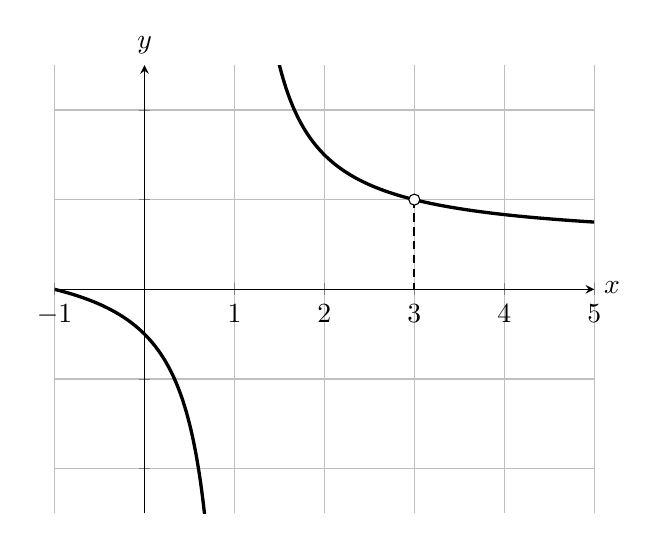
\begin{tikzpicture}
	\begin{axis}
	[ymin=-5,ymax=5, axis lines=center,xlabel=$x$,ylabel=$y$,every axis y 
	label/.style={at=(current axis.above origin),anchor=south},every axis x label/.style={at=(current axis.right of origin),anchor=west},
	domain=-1:5,
	yticklabels={},
	ymajorgrids=true,
	grid = major
	]
	\addplot[domain=-1:99/100,very thick,smooth,samples=500]
	{(\x^2-2*\x-3)/(\x^2-4*\x+3)};
	\addplot[domain=101/100:5,very thick,smooth,samples=500]
	{(\x^2-2*\x-3)/(\x^2-4*\x+3)};
	\draw[densely dashed, thick] (axis cs:3,2)--(axis cs:3,0);
	\draw[fill=white] (axis cs:3,2) circle [radius=2pt];
	\end{axis}
       \end{tikzpicture}      
      \end{center}
      There is a removable discontinuity at $x=3$. This suggests something about the factorization of both polynomials $x^2-2x-3$ and $x^2-4x+3$.
    \end{hint}
    \begin{hint}
     Notice that the quadratic equation tells us that $x^2-2x-3=0$ has solutions $1\pm2$ and $x^2-4x+3=0$ has solutions $2\pm{1}$. Thus, $x^2-2x-3=\left(x-3\right)\left(x+1\right)$ and $x^2-4x+3=\left(x-3\right)\left(x-1\right)$. Then $\lim\limits_{x\to3}\frac{x^2-2x-3}{x^2-4x+3}=\lim\limits_{x\to3}\frac{x+1}{x-1}$. 
    \end{hint}
    \answer{$2$}.
  \end{solution}
\end{question}

\end{document}